% ======================================================================
\section{Results}\label{sec:results}

This section presents the results in the order of the research questions. \Cref{sec:res-config} describes where countries stand relative to the social foundation and the climate boundary, and how this changed over time. \Cref{sec:res-cross} examines the countries that crossed the social foundation. \Cref{sec:res-req} presents the carbon requirement and \cref{sec:res-frontier} the countries that met the foundation with the least carbon. \Cref{sec:res-within} reports the within-country evidence, \cref{sec:res-decoupling} the decoupling analysis and \cref{sec:res-persist} the persistence of the configurations. \Cref{sec:res-robust} closes with the robustness analysis, distinguishing results that are stable across specifications from estimates whose level depends on them.

\subsection{Shortfall and overshoot, \nFirstYear--\nLastYear}\label{sec:res-config}

\Cref{fig:space} shows each country in the main sample in 2011--2022. The horizontal axis shows its consumption-based \COtwo{} emissions per person on a logarithmic scale, and the vertical axis its weakest social attainment ratio. A value of one on the vertical axis means all four social thresholds are met. The dashed vertical line marks the climate boundary.

The figure shows the central result of the paper: the safe and just space in the upper left is empty. This holds not only for the period averages but for every individual year: among the \nNCons{} countries with consumption-based emissions, the number of country-years classified as safe and just between \nShareYearStart{} and \nLastYear{} is \nNEverSafeYears. Countries that meet all four thresholds emitted between \nFrontierMin~t (\nFrontierMinCountry) and \nMetMaxCons~t (\nMetMaxCountry) of \COtwo{} per person, all above the boundary. Countries within the boundary all fall short on at least one indicator, often by a wide margin. In the lower left are countries such as Ethiopia, Nigeria and Pakistan. For each of them the weakest indicator is under-5 mortality, and it reaches less than half of its threshold. Between these two groups lies a large set of countries that are close to meeting the foundation. \nNearN{} countries are within 10\% of every threshold without meeting all of them, \nNearEurope{} of them in Europe and \nNearAmerica{} in the Americas. Their median emissions are \nNearMedianMultiple{} times the boundary.

\begin{figure}[tbp]
\centering
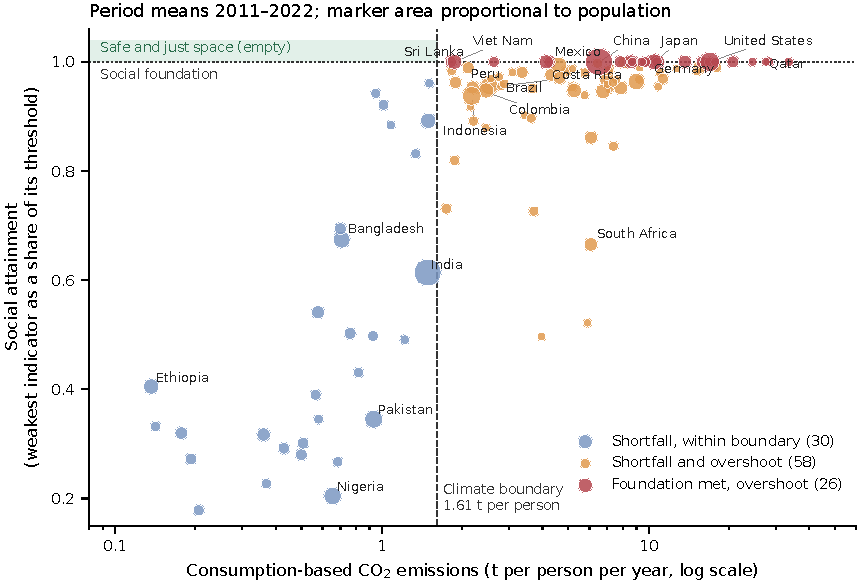
\includegraphics[width=\textwidth]{../figures/fig1_space.pdf}
\caption{Social attainment and consumption-based \COtwo{} emissions, 2011--2022 period means. The vertical axis shows each country's weakest social indicator relative to its threshold (1 means all four thresholds are met). The dashed line marks the \nBoundary~t climate boundary and the dotted line the social foundation. Marker area is proportional to population. Counts in the legend are numbers of countries.}
\label{fig:space}
\end{figure}

\Cref{tab:counts} counts the countries in each configuration in each period. Between 1990--2000 and 2011--2022, the number falling short within the boundary declined, the number meeting the foundation while overshooting more than doubled, and the number in the safe and just space was zero in every period. The largest group in every period was the countries that both fall short and overshoot.

\begin{table}[tbp]
\centering
\small
\caption{Countries in each configuration, by period (period means, consumption-based CO$_2$).}
\label{tab:counts}
\begin{threeparttable}
\begin{tabular}{lrrrrr}
\toprule
Period & Shortfall, within & Shortfall, overshoot & Met, overshoot & Safe and just & Total \\
\midrule
1990–2000 & 47 & 55 & 11 & 0 & 113 \\
2001–2010 & 40 & 53 & 21 & 0 & 114 \\
2011–2022 & 30 & 58 & 26 & 0 & 114 \\
\bottomrule
\end{tabular}
\begin{tablenotes}[flushleft]
\footnotesize
\item \textit{Notes:} Foundation met: all four social indicators at or beyond their thresholds. Overshoot: consumption-based CO$_2$ above 1.61 t per person.
\end{tablenotes}
\end{threeparttable}
\end{table}


\Cref{fig:shares} tracks the configurations year by year from \nShareYearStart. To ensure that changes reflect countries' outcomes rather than countries entering or leaving the data, the figure uses a balanced panel of the \nBalancedN{} countries that can be classified in every year. In panel (a), each country counts equally. The share meeting the social foundation rose from \nMetStart\% in \nShareYearStart{} to \nMetEnd\% in \nLastYear. The share overshooting the climate boundary rose from \nOverStart\% to \nOverEnd\%. The share falling short within the boundary declined from \nShareWithinStart\% to \nShareWithinEnd\%, and the share both falling short and overshooting from \nShareTrapStart\% to \nShareTrapEnd\%. The safe and just share was zero in every year.

\begin{figure}[tbp]
\centering
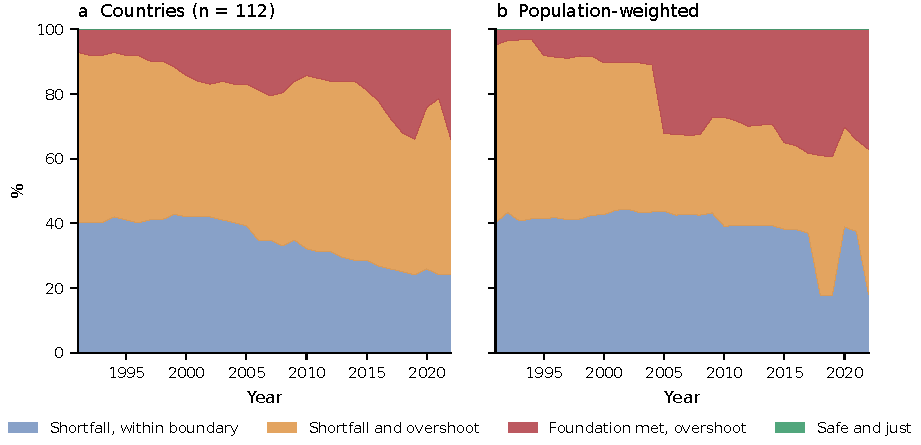
\includegraphics[width=\textwidth]{../figures/fig2_shares.pdf}
\caption{Configurations of shortfall and overshoot, \nShareYearStart--\nLastYear. (a)~Share of countries in a balanced panel (countries classified in every year). (b)~Share of the population of the same countries.}
\label{fig:shares}
\end{figure}

Panel (b) weights each country by its population, which changes the picture considerably because a few countries are very large. The share of people living in countries that meet the foundation while overshooting rose from \nPopOverStart\% to \nPopOverEnd\%. The share living in countries that both fall short and overshoot fell from \nPopTrapStart\% to \nPopTrapEnd\%, and the share in countries falling short within the boundary from \nPopWithinStart\% to \nPopWithinEnd\%. Two countries drive the large steps in this series. China has met the social foundation in every year since \nChinaFirstMet, moving \nChinaPopShare\% of the population in the panel into the ``foundation met, overshoot'' configuration. India's consumption-based emissions first exceeded the boundary in \nIndiaFirstOver{} and stood at \nIndiaEndCons~t per person in \nLastYear, very close to the boundary. India's 1.4 billion people therefore move between ``shortfall within'' and ``shortfall and overshoot'' as its emissions cross \nBoundary~t from one year to the next. This sensitivity illustrates a general point. For countries near the boundary, the classification of a single year is fragile, and the trajectory over several years is more informative.

\subsection{Crossing the social foundation}\label{sec:res-cross}

The configurations describe positions. A more direct test of whether development can run through the safe and just space is to follow the countries that crossed the social foundation during the period. \nNCrossers{} countries started the period below the social foundation and met it at some later point. For each of them, the year in which it first met the foundation was identified, along with whether its emissions were above or below the boundary in that year.

All \nNCrossersAbove{} of them were above the climate boundary when they first met the foundation. Their median consumption-based emissions in that year were \nCrossCarbonMedian~t per person, \nCrossCarbonMultiple{} times the boundary.

Because social indicators fluctuate from year to year, particularly employment, a country can meet the foundation in a single year and then fall back. A stricter definition of crossing requires the foundation to be met in three consecutive years, and dates the crossing to the first of them. Under this definition \nNCrossersSust{} countries crossed, and all \nNCrossersSustAbove{} of them were above the boundary at the time, at a median of \nCrossSustCarbonMedian~t per person. No country crossed the social foundation from within the boundary. The typical historical path ran from shortfall within the boundary, through a period of shortfall with overshoot as emissions rose, to meeting the foundation above the boundary. This is the path sketched by the arrow in \cref{fig:framework}.

\subsection{The carbon requirement}\label{sec:res-req}

\Cref{fig:requirement} shows the carbon requirement: the consumption-based \COtwo{} per person at which half of countries meet the social foundation. The points are annual estimates, each from a separate cross-sectional logit. The lines and shaded bands are the pooled model with its 95\% country-cluster bootstrap interval.

\begin{figure}[tbp]
\centering
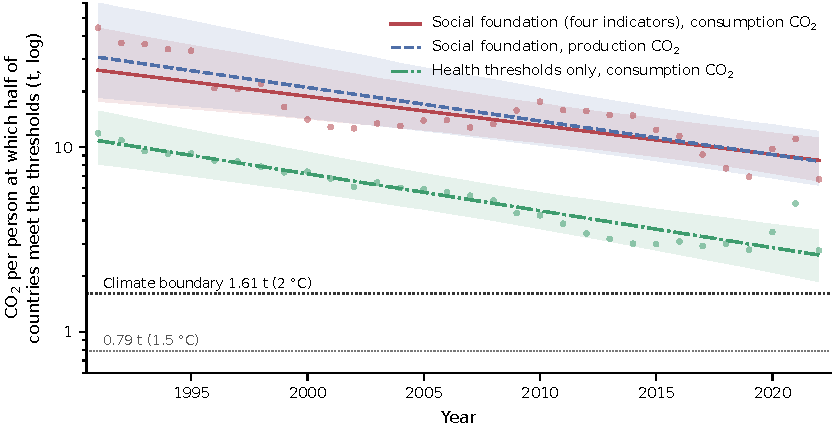
\includegraphics[width=\textwidth]{../figures/fig3_requirement.pdf}
\caption{The carbon requirement: \COtwo{} per person at which half of countries meet the thresholds. Points are annual cross-sectional logit estimates. Lines and shaded bands are the pooled model with 95\% country-cluster bootstrap intervals (\nBootReps{} replications). Health thresholds: life expectancy $\geq$ 74 years and under-5 mortality $\leq$ 25. The rise in 2020--2021 coincides with the falls in life expectancy and employment during the COVID-19 pandemic.}
\label{fig:requirement}
\end{figure}

\paragraph{Main estimate.} In the pooled model, the requirement fell from about \nReqStart~t per person in \nShareYearStart{} (95\% CI \nReqStartLo--\nReqStartHi) to \nReqMid~t in 2000 and \nReqEnd~t in \nLastYear{} (\nReqEndLo--\nReqEndHi). This is an average decline of \nReqTrend\% a year (95\% CI \nReqTrendLo--\nReqTrendHi), a fall by a factor of \nReqFactor{} over three decades. The annual estimate for \nLastYear{} alone is \nReqAnnualEnd~t, somewhat below the pooled value. The annual estimates suggest the decline was faster in the late 2010s than the constant rate assumed by the pooled model, interrupted by the pandemic in 2020--2021.

However measured, the requirement remained far above the boundary. In \nLastYear{} the pooled estimate was \nReqEndMultiple{} times the 2\textdegree C boundary and \nReqEndFifteenMultiple{} times the 1.5\textdegree C value. Even the lower end of its confidence interval was well above both.

\paragraph{Health thresholds alone.} The requirement for the two health thresholds, life expectancy and under-5 mortality, was much lower and fell faster. It went from \nReqHealthStart~t in \nShareYearStart{} to \nReqHealthEnd~t in \nLastYear{} (95\% CI \nReqHealthEndLo--\nReqHealthEndHi), a decline of \nReqTrendHealth\% a year. Meeting the full foundation is therefore associated with several times more carbon than meeting the health thresholds alone. The difference is attributable to electricity access and employment, the two dimensions most closely tied to economic structure and energy systems. The health requirement in \nLastYear{} was within a factor of two of the boundary.

\paragraph{Production-based emissions.} With production-based emissions, for all \nNCountries{} countries, the requirement was \nReqProdEnd~t in \nLastYear{} and fell by \nReqTrendProd\% a year, very close to the consumption-based estimate. The result is therefore not an artefact of how emissions embodied in trade are allocated.

\paragraph{Fit diagnostics.} None of the \nReqYearsMain{} annual point estimates or the pooled point estimate failed. Of the \nReqBootTotalMain{} annual bootstrap replications in the main specification, \nReqBootFailMain{} failed, at most \nReqBootFailMaxMain\% in any single year. The worst year was \nReqBootFailWorstYear{} (\nReqBootFailWorstReasons). Failures are concentrated in years when few countries met the foundation, so that some bootstrap samples contained too few such countries to fit the curve. Among the \nBootReps{} pooled bootstrap replications, the number that failed was \nPooledBootFailMain. The failed fits are too few to affect the confidence intervals. \Cref{tab:reqannual} in \cref{app:extra} lists every annual estimate with its interval and number of failed replications.

\subsection{Countries at the frontier}\label{sec:res-frontier}

The requirement describes the typical relationship across countries. Individual countries vary widely around it. \Cref{tab:frontier} lists the ten countries that met the social foundation with the lowest consumption-based emissions in 2011--2022.

\begin{table}[tbp]
\centering
\small
\caption{The ten lowest-carbon countries meeting the social foundation, 2011–2022.}
\label{tab:frontier}
\begin{threeparttable}
\begin{tabular}{lrrrrr}
\toprule
Country & CO$_2$ (t) & $\times$ boundary & Life exp. & U5MR & Lowest ratio \\
\midrule
Sri Lanka & 1.81 & 1.1 & 76.1 & 8.3 & 1.00 \\
Viet Nam & 1.87 & 1.2 & 74.1 & 21.7 & 1.00 \\
Ecuador & 2.63 & 1.6 & 75.6 & 15.1 & 1.00 \\
Thailand & 4.13 & 2.6 & 76.5 & 11.4 & 1.00 \\
Romania & 4.25 & 2.6 & 74.8 & 8.6 & 1.00 \\
China & 6.51 & 4.0 & 77.2 & 10.0 & 1.00 \\
Malaysia & 7.83 & 4.9 & 75.4 & 8.1 & 1.00 \\
United Kingdom & 8.61 & 5.3 & 81.0 & 4.5 & 1.00 \\
New Zealand & 8.67 & 5.4 & 81.7 & 5.4 & 1.00 \\
Norway & 9.42 & 5.8 & 82.4 & 2.6 & 1.00 \\
\bottomrule
\end{tabular}
\begin{tablenotes}[flushleft]
\footnotesize
\item \textit{Notes:} Period means of consumption-based CO$_2$ per person. U5MR: under-5 mortality per 1,000 live births. Lowest ratio: the weakest social indicator relative to its threshold.
\end{tablenotes}
\end{threeparttable}
\end{table}


\nFrontierMinCountry{} met the foundation at \nFrontierMin~t per person, only \nFrontierMinMultiple{} times the boundary. It was followed by Viet Nam and Ecuador. Beyond these three, the next lowest emitter meeting the foundation emitted \nFrontierFourth~t. So a small number of countries have come close to meeting basic needs within the climate boundary, at about two tonnes per person. That is roughly a quarter of the typical requirement in \nLastYear{} (\nReqAnnualEnd~t in the annual estimate and \nReqEnd~t in the pooled model). The width of this range, from about two tonnes at the frontier to \nMetMaxCons~t at the top, shows how differently countries convert emissions into social outcomes. That variation is consistent with the evidence that the way basic services are provided shapes the energy needed to provide them \citep{vogel2021}.

This paper does not test which characteristics explain why these countries meet the foundation with relatively little carbon. That would require detailed case studies of their energy systems and social provision. The list of ten is also sensitive to the exact thresholds: countries just above a threshold enter it, and countries just below do not.

\subsection{Within-country evidence}\label{sec:res-within}

\Cref{tab:fe} reports the two-way fixed-effects estimates of \cref{eq:fe}. Each cell gives the coefficient on log emissions per person: the association between changes in a country's emissions and changes in its outcome, net of the country's own average and of the global trend in each year.

\begin{table}[tbp]
\centering
\small
\caption{Within-country association between log emissions per person and social outcomes.}
\label{tab:fe}
\begin{threeparttable}
\begin{tabular}{llrrr}
\toprule
Pressure & Outcome & Without income & With log GDP & N \\
\midrule
Consumption CO$_2$ & Life expectancy (years) & 1.563$^{***}$ (0.362) & 1.395$^{***}$ (0.367) & 3,748 \\
 & Social attainment (0--1) & 0.069$^{***}$ (0.012) & 0.065$^{***}$ (0.012) & 3,724 \\
Production CO$_2$ & Life expectancy (years) & 1.632$^{***}$ (0.337) & 1.446$^{***}$ (0.365) & 4,916 \\
 & Social attainment (0--1) & 0.063$^{***}$ (0.010) & 0.063$^{***}$ (0.010) & 4,866 \\
GHG incl.\ land use & Life expectancy (years) & 0.242 (0.350) & -0.073 (0.357) & 4,884 \\
 & Social attainment (0--1) & 0.008 (0.008) & -0.008 (0.008) & 4,835 \\
\bottomrule
\end{tabular}
\begin{tablenotes}[flushleft]
\footnotesize
\item \textit{Notes:} Coefficients on log emissions per person from two-way fixed-effects models (country and year effects); standard errors clustered by country in parentheses. $^{*}p<0.05$, $^{**}p<0.01$, $^{***}p<0.001$.
\end{tablenotes}
\end{threeparttable}
\end{table}


With consumption-based emissions and controlling for income, a 10\% rise in emissions per person is associated with a \nFeLETen-year rise in life expectancy, and a doubling with \nFeLEDouble{} years ($\hat\beta$ = \nFeLE, s.e.\ \nFeLESe; \nFeN{} country-years in \nFeCountries{} countries). The association is statistically significant but small. For comparison, mean life expectancy in these countries rose by \nLeGain{} years over the period, from \nLeStart{} in \nShareYearStart{} to \nLeEnd{} in \nLastYear{}, while median consumption-based emissions per person rose from \nDescCOFirst~t to \nDescCOLast~t between the first and last periods (\cref{tab:desc}). Results with production-based emissions are very similar. With total greenhouse gases including land use as the pressure measure, there is no association ($p$ = \nFeGhgP).

The long-difference regressions (\cref{tab:longdiff} in \cref{app:extra}) relate the change in each outcome between 1990--2000 and 2011--2022 to the change in log emissions and income over the same interval. For life expectancy they show no association with emissions once income growth is controlled for ($\hat\beta$ = \nLdLE, $p$ = \nLdLEP, $N$ = \nLdN), while income growth itself remains significant. For mean social attainment, which includes electricity access, the association with emissions is positive and significant.

The two estimators therefore disagree on life expectancy. Annual fixed effects show a small positive association, and long differences show none. Both are consistent with emissions growth having accounted, net of income, for at most a small part of the health gains of the period. The association is clearer for the broader social attainment measure, which includes access to electricity, the dimension most directly tied to energy use. Neither estimator identifies causal effects, for the reasons given in \cref{sec:methods}.

\subsection{Decoupling}\label{sec:res-decoupling}

\Cref{tab:decoupling} classifies countries by the relationship between the trends in their consumption-based emissions and their income per person.

\begin{table}[tbp]
\centering
\small
\caption{Decoupling of consumption-based CO$_2$ per person from GDP per person.}
\label{tab:decoupling}
\begin{threeparttable}
\begin{tabular}{lrrrrrr}
\toprule
Window & Absolute & Relative & Coupled & No growth & Absolute (CI $<$ 0) & N \\
\midrule
2001--2010 & 24 & 58 & 29 & 3 & 6 & 114 \\
2011--2022 & 48 & 27 & 23 & 16 & 34 & 114 \\
\bottomrule
\end{tabular}
\begin{tablenotes}[flushleft]
\footnotesize
\item \textit{Notes:} Annual growth rates from log-linear trends. Absolute: income rising, emissions falling. Relative: both rising, emissions more slowly. Coupled: emissions rising at least as fast as income. The last column requires the 95\% confidence interval of the emissions trend to lie below zero.
\end{tablenotes}
\end{threeparttable}
\end{table}


Absolute decoupling became much more common. In 2001--2010, \nDecAbsEarly{} countries had falling emissions while their incomes grew. In 2011--2022 the number was \nDecAbsLate, and in \nDecAbsLateRobust{} of them the emissions trend was significantly below zero. Another \nDecRelLate{} countries decoupled relatively in 2011--2022, with emissions growing more slowly than income. \nDecCoupledLate{} countries remained coupled, and \nDecNoGrowthLate{} had no income growth over the decade, so their emission trends cannot be interpreted as decoupling. The absolute decouplers include the United States, Japan, most of Western Europe and several middle-income countries in Latin America and Eastern Europe. Life expectancy rose in \nDecLEUp{} of the \nDecAbsLate{} absolute decouplers, so falling emissions did not, in general, go with a deterioration in health.

The problem is speed. \nDecAbsBelow{} of the absolute decouplers were already within the boundary. \Cref{fig:decoupling} compares achieved and required rates for the remaining \nDecAbsAbove. Only \nDecAboveOnTrack{} of them (\nDecAboveOnTrackList) cut emissions fast enough to reach \nBoundary~t per person by 2050. The median decoupler cut emissions by \nDecMedianAchieved\% a year, against \nDecMedianRequired\% required. The required rate was \nDecSpeedRatio{} times the achieved one. Even \nDecFastest, the fastest decoupler, cut emissions by \nDecFastestRate\% a year against \nDecFastestRequired\% required. At their achieved rates, the median decoupler would need \nDecMedianYears{} years to reach the boundary.

\begin{figure}[tbp]
\centering
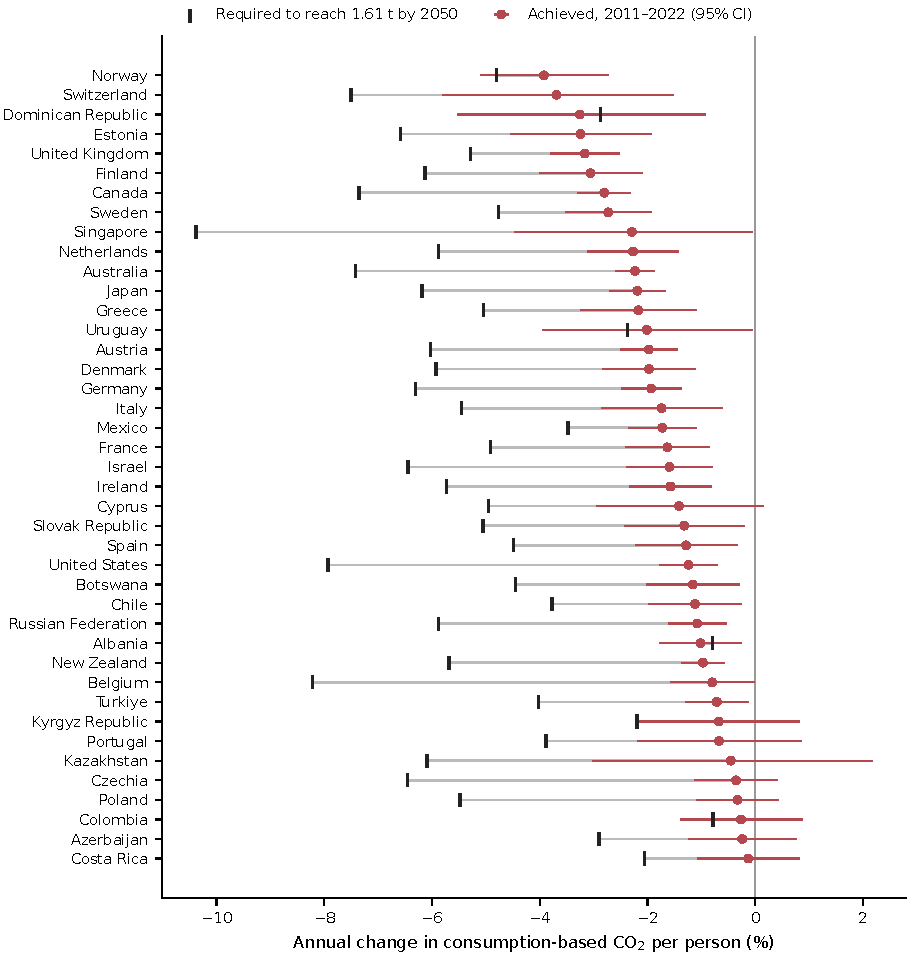
\includegraphics[width=0.92\textwidth]{../figures/fig4_decoupling.pdf}
\caption{Achieved and required change in consumption-based \COtwo{} per person, 2011--2022, for the \nDecAbsAbove{} absolute decouplers above the boundary. Dots show the achieved annual change with its 95\% confidence interval from a log-linear trend. Ticks show the constant annual change required to reach \nBoundary~t by 2050 from the \nLastYear{} level.}
\label{fig:decoupling}
\end{figure}

\Cref{tab:scenarios} shows how this conclusion depends on the assumption that achieved rates continue. If every country doubled its achieved rate, \nScenDouble{} of the \nDecAbsAbove{} would reach the boundary by 2050. If all achieved the 90th-percentile rate of the group (\nScenNinetyRate\% a year), \nScenNinety{} would. Even if every country matched the fastest rate any of them achieved (\nScenFastestRate\% a year), only \nScenFastest{} would arrive in time. Under achieved rates the median country would reach the boundary around \nScenAchievedYear; under doubled rates, around \nScenDoubleYear. Reaching the boundary by 2050 would require each country to cut emissions at its own required rate, faster than any country in the group has managed over a decade.

\begin{table}[tbp]
\centering
\small
\caption{Illustrative scenarios for the absolute decouplers above the boundary.}
\label{tab:scenarios}
\begin{threeparttable}
\begin{tabular}{lrrr}
\toprule
Scenario & Median cut (\%/yr) & Reach 1.61 t by 2050 & Median year reached \\
\midrule
Achieved 2011--2022 rates & 1.6 & 2 of 41 & 2115 \\
Each country doubles its rate & 3.2 & 6 of 41 & 2068 \\
All at the 90th-percentile rate & 3.2 & 7 of 41 & 2071 \\
All at the fastest achieved rate & 3.9 & 10 of 41 & 2061 \\
Each at the rate required by 2050 & 5.5 & 41 of 41 & 2050 \\
\bottomrule
\end{tabular}
\begin{tablenotes}[flushleft]
\footnotesize
\item \textit{Notes:} Each scenario applies a constant annual rate of change in consumption-based CO$_2$ per person from each country's 2022 level. The 90th-percentile and fastest rates are those achieved by this group in 2011--2022. These are arithmetic illustrations, not forecasts.
\end{tablenotes}
\end{threeparttable}
\end{table}


\subsection{Persistence of the configurations}\label{sec:res-persist}

\Cref{fig:transitions} shows how countries moved between configurations from one period to the next. Most countries stayed where they were: \nPersistOne\% remained in the same configuration between 1990--2000 and 2001--2010, and \nPersistTwo\% between 2001--2010 and 2011--2022.

\begin{figure}[tbp]
\centering
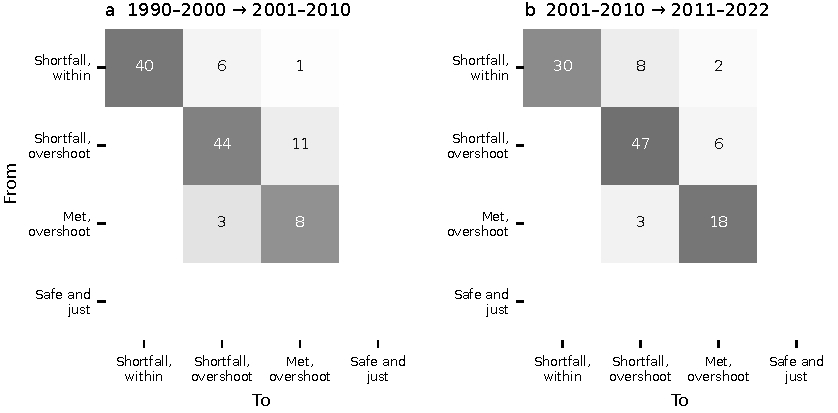
\includegraphics[width=0.92\textwidth]{../figures/fig5_transitions.pdf}
\caption{Transitions between configurations across periods (number of countries, period means). Shading shows the share of each origin row. The safe and just row and column are empty.}
\label{fig:transitions}
\end{figure}

The movements that did occur ran almost entirely in one direction, towards higher social attainment and higher emissions. Of the \nWithinTotal{} countries falling short within the boundary in 2001--2010, \nWithinStay{} remained there by 2011--2022. \nWithinToTrap{} crossed into overshoot while still falling short, and \nWithinToOver{} reached the foundation above the boundary. Of the \nTrapTotal{} countries that both fell short and overshot, \nTrapToOver{} reached the foundation. No country entered the safe and just space in either transition (\nIntoSafe{} such moves).

As a check that does not rely on the thresholds, Gaussian mixture models were fitted to log emissions and mean social attainment for the \nGmmN{} classified country-periods. The Bayesian information criterion selects \nGmmK{} components (\cref{fig:gmm} in \cref{app:extra}). The four-component solution agrees moderately with the threshold-based configurations (adjusted Rand index \nGmmAri) and is moderately stable across bootstrap samples (median adjusted Rand index \nGmmStab). The data do not split into sharply separated groups. They form a gradient along which social attainment and emissions rise together, and the threshold-based configurations divide that gradient at substantively meaningful points.

\subsection{Robustness}\label{sec:res-robust}

\Cref{tab:robustness} repeats the headline results under each alternative specification described in \cref{sec:robust}. \Cref{tab:stability} summarises which conclusions are stable and which quantities change.

\begin{table}[tbp]
\centering
\footnotesize
\setlength{\tabcolsep}{3.5pt}
\caption{Headline results under alternative specifications.}
\label{tab:robustness}
\begin{threeparttable}
\begin{tabular}{lrrrrrrr}
\toprule
Specification & N & Met (\%) & Over (\%) & Safe \& just & Lowest t & Req.\ (t) & Decline (\%/yr) \\
\midrule
Main specification & 114 & 34 & 76 & 0 & 1.8 & 8.5 & 3.6 \\
Production-based CO$_2$ & 155 & 26 & 61 & 1 & 0.9 & 8.4 & 4.1 \\
Production-based, same countries & 114 & 34 & 70 & 1 & 0.9 & 7.5 & 4.4 \\
1.5\textdegree C boundary (0.79 t) & 114 & 34 & 87 & 0 & 1.8 & 8.5 & 3.6 \\
Within 5\% of every threshold & 113 & 65 & 76 & 1 & 1.5 & 2.3 & 4.7 \\
Mean attainment $\geq$ 0.95 & 113 & 35 & 76 & 0 & 1.8 & 8.5 & 3.5 \\
Adding secondary enrolment (5) & 112 & 26 & 76 & 0 & 2.6 & 9.0 & 5.1 \\
Without employment (3) & 114 & 57 & 76 & 0 & 1.8 & 2.9 & 4.2 \\
No interpolation or gap filling & 114 & 34 & 76 & 0 & 1.8 & 8.4 & 3.6 \\
\bottomrule
\end{tabular}
\begin{tablenotes}[flushleft]
\footnotesize
\item \textit{Notes:} Met and Over: shares of countries in 2022 meeting the social foundation and overshooting the boundary. Safe \& just: countries in that configuration in the 2011–2022 (period means). Lowest t: lowest per-capita CO$_2$ among countries meeting the foundation in that period. Req.: CO$_2$ per person at which half of countries meet the foundation in 2022 and Decline: its average annual fall, both from the pooled logit model (Section~\ref{sec:methods}).
\end{tablenotes}
\end{threeparttable}
\end{table}


\begin{table}[tbp]
\centering
\small
\caption{Which results are stable across specifications and which are not.}
\label{tab:stability}
\begin{threeparttable}
\begin{tabular}{>{\raggedright\arraybackslash}p{0.5\linewidth}rrr}
\toprule
Result & Main & Range & Holds in \\
\midrule
No country in the safe and just space, 2011--2022 & 0 & 0--1 & 6 of 9 \\
Requirement above the 2\textdegree C boundary in 2022 (t) & 8.5 & 2.3--9.0 & 9 of 9 \\
Requirement falling (\% per year, 95\% CI below 0) & 3.6 & 3.5--5.1 & 9 of 9 \\
Share of countries meeting the foundation, 2022 (\%) & 34 & 26--65 & level varies \\
Share of countries overshooting, 2022 (\%) & 76 & 61--87 & level varies \\
Lowest CO$_2$ among countries meeting the foundation (t) & 1.8 & 0.9--2.6 & level varies \\
\bottomrule
\end{tabular}
\begin{tablenotes}[flushleft]
\footnotesize
\item \textit{Notes:} Range across the specifications of Table~\ref{tab:robustness}. ``Level varies'' marks quantities whose value depends on the specification even though the qualitative conclusion does not.
\end{tablenotes}
\end{threeparttable}
\end{table}


Three conclusions hold in every specification. First, the safe and just space in 2011--2022 contains no country in \nRobSafeZeroSpecs{} of the \nRobSpecs{} specifications and never more than \nRobSafeMax. Second, the carbon requirement in \nLastYear{} lies above the boundary in every specification, ranging from \nRobReqMin~t to \nRobReqMax~t. Third, the requirement falls in every specification, by \nRobTrendMin\% to \nRobTrendMax\% a year, with confidence intervals that exclude zero in \nRobTrendAllNeg{} specifications.

The level of the requirement, in contrast, depends strongly on how the social foundation is defined. Tolerating a 5\% shortfall on each indicator lowers it to \nRobReqTol~t, and dropping employment lowers it to \nRobReqNoEmp~t. Adding secondary enrolment raises it to \nRobReqEdu~t. A more demanding foundation is associated with more carbon, as one would expect. The level of the requirement should therefore always be read together with the thresholds that define it, and the paper treats its decline and its position above the boundary as the robust findings. The shares of countries meeting the foundation and overshooting also vary across specifications, while the direction of change in both does not.

The safe and just cases that appear in alternative specifications are informative. With production-based emissions, \nProdSafeList{} appears in the safe and just space in 2011--2022. Its territorial emissions (\nProdSafeProd~t) are within the boundary, but its consumption-based emissions (\nProdSafeCons~t) are not. The difference reflects emissions embodied in imports. Year by year, production-based emissions place \nProdSafeCountriesAll{} in the safe and just space in \nProdSafeYearsAll{} country-years in total, and in each of those years the country's consumption-based emissions exceeded the boundary. The \nMissOutN{} countries without consumption-based estimates are never in the safe and just space on the production-based measure (\nNoConsSafeYears{} of \nNoConsClassifiedYears{} classified country-years). Removing all interpolation and gap filling changes the results only marginally. The emptiness of the safe and just space on a consumption basis does, however, depend on applying the thresholds strictly. When each indicator may fall up to 5\% short of its threshold, \nRobTolSafePeriod{} is in the safe and just space in 2011--2022, and \nRobTolSafeYear{} are there in \nLastYear. These countries have low emissions and come close to, but do not reach, all four thresholds.
